\section{Results in the Rotated Basis}\label{sec:eft_rotated_basis_results}

Given that BSM theories usually predict a variety of new physics effects, e.g.\ more than one new particle and/or interaction, it is expected that multiple Wilson coefficients will be non-zero. If that's the case, then the individual constraints in the nominal basis from \cref{sec:eft_nominal_basis_results} are not valid if one wants to draw a comparison with the predictions from a BSM theory. Instead, one needs to constrain the Wilson coefficients simultaneously. Here, this means providing constraints on Wilson coefficients when leaving the other coefficients freely floating in the fit, i.e.\ when making no assumption about their values. 

The data available in this combination is not sufficient to constrain all 43 Wilson coefficients simultaneously since some Wilson coefficients have nearly degenerate effects on the observables, leading to flat directions in the likelihood. This is illustrated in some 2D toy examples in \cref{fig:pca_toy}, where in the first example, both coefficients, $C_i$ and $C_j$, can be simultaneously constrained, but in the second example, there is a flat direction along the line $C_i = -C_j$. In this case, the linear combination of coefficients, $C_0 = C_i + C_j$, can be constrained, but the combination, $C_1 = C_i - C_j$, cannot. 

\begin{figure}
  \centering
  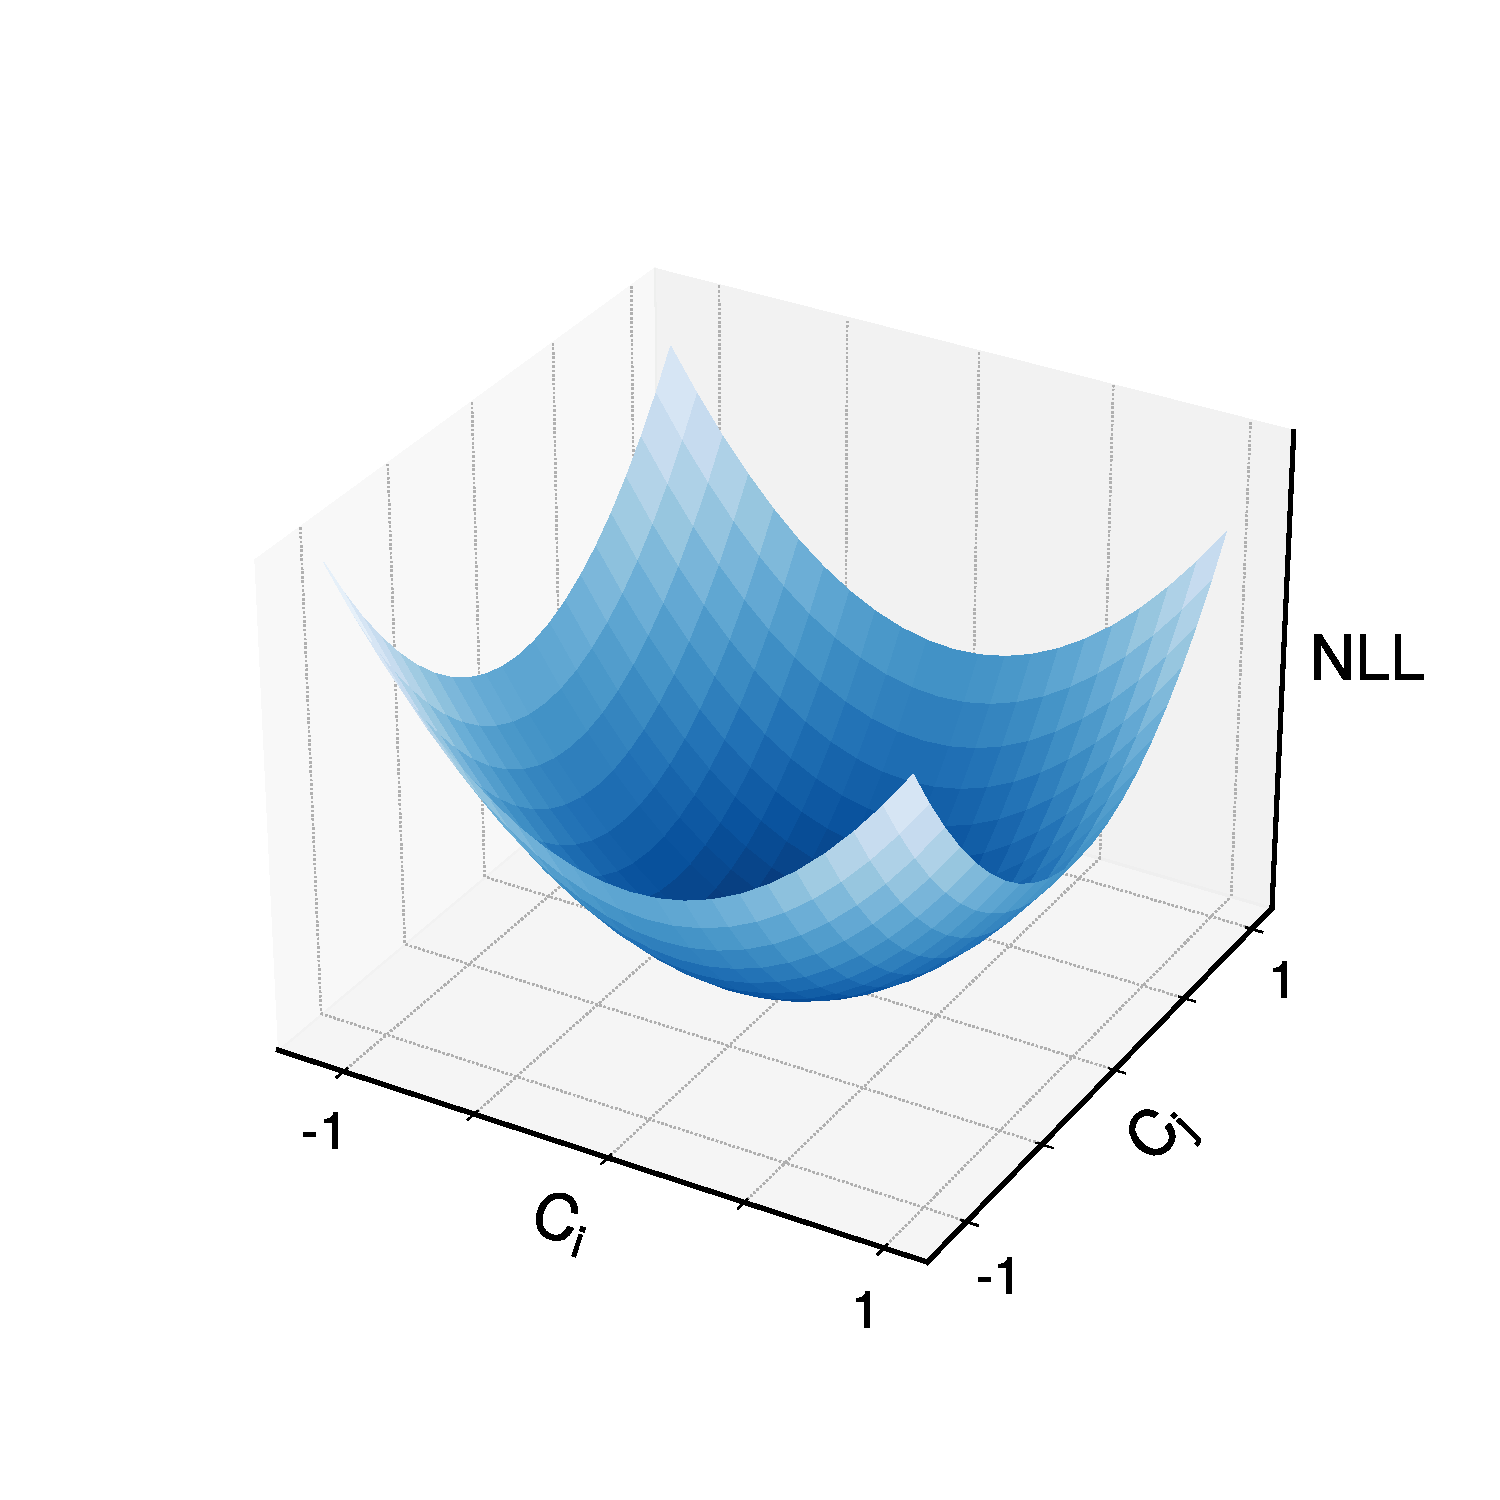
\includegraphics[width=0.49\textwidth]{Figures/EFT/pca_toy_a.pdf}
  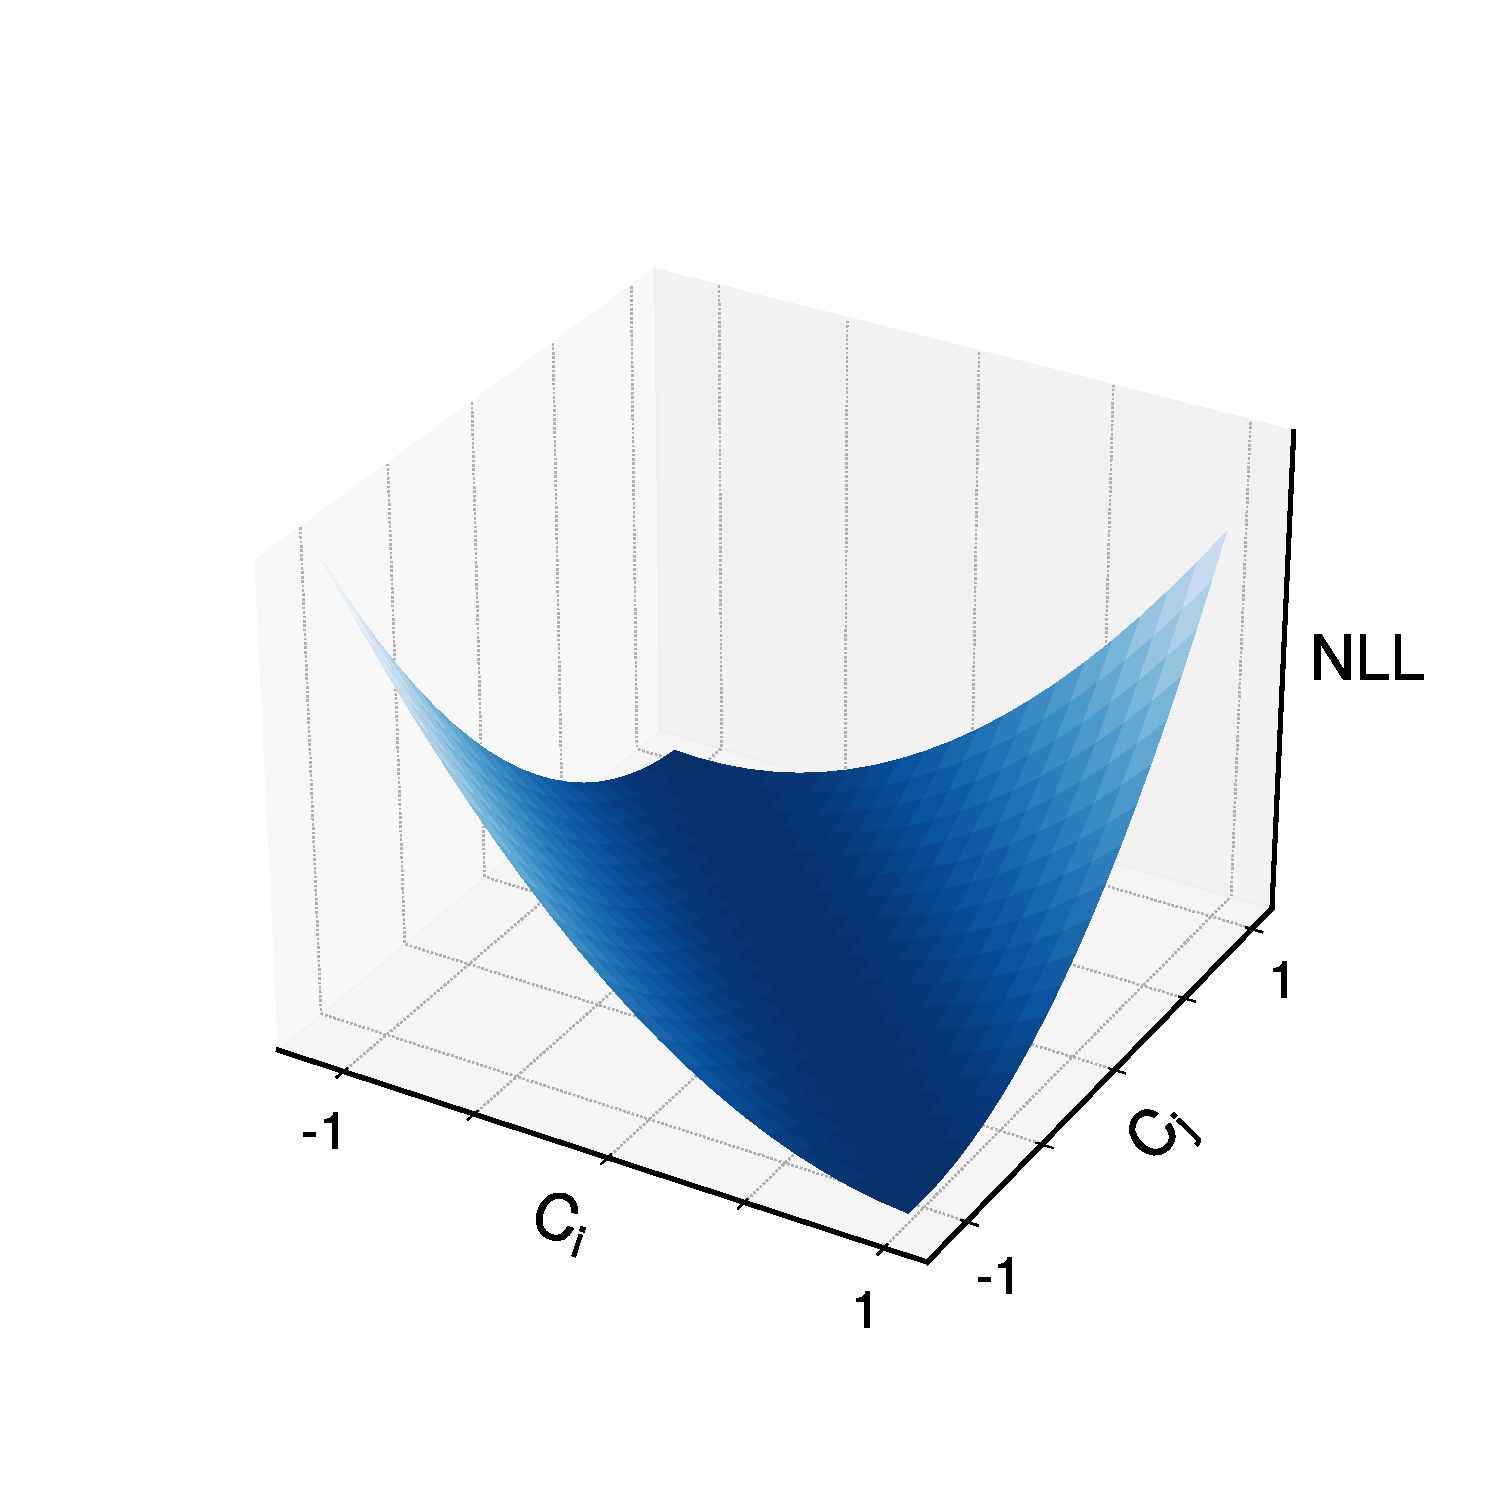
\includegraphics[width=0.49\textwidth]{Figures/EFT/pca_toy_b.pdf}
  \caption[PCA Illustration]{Two illustrative examples of a negative log likelihood (NLL) surface in two dimensions. On the left, the surface represents a scenario where it is possible to constrain both Wilson coefficients, $C_i$ and $C_j$ simultaneously. On the right, there is a flat direction along $C_i = -C_j$ meaning neither coefficient can be constrained whilst leaving the other floating. However, a linear combination, $C_0=C_i+C_j$ is able be constrained which corresponds to the direction perpendicular to the flat direction.}\label{fig:pca_toy}
\end{figure}

In the 43-dimensional case, the idea is the same, and the curvature of the log-likelihood function is studied at its minimum to determine which directions are flat, and which directions are sensitive to the data (the rotated basis). This is formalized in a principal component analysis technique which derives the directions from $\mathcal{H}_{\text{SMEFT}}$, which is the Hessian matrix corresponding to the second derivatives of the negative log likelihood (NLL) with respect to the Wilson coefficients, evaluated at the NLL minimum. When using the linear-plus-quadratic parameterization, this matrix is a function of the Wilson coefficients. Since the values of the coefficients are not known a priori, they are set to zero for the sake of deriving the rotated basis, which is equivalent to using the linear parameterization only.

An eigenvector decomposition is used to write $\mathcal{H}_{\text{SMEFT}} = \mathcal{R}^T \Lambda \mathcal{R}$ where $\mathcal{R}$ is a rotation matrix that defines the linear combinations of Wilson coefficients (the eigenvectors) via $\text{EV}_j = \sum_k \mathcal{R}_{jk} C_k$, and $\Lambda$ is a diagonal matrix containing the corresponding eigenvalues, $\lambda_i$, which indicate the constraining power for each eigenvector where the expected 68\% CL interval is given by $1 / \sqrt{\lambda_i}$. In the fit, combinations of Wilson coefficients with $1/\sqrt{\lambda_i} > 10$ are set to zero, therefore removing flat (or approximately flat) directions in the likelihood, and the 17 remaining eigenvectors, shown in \cref{fig:pca_rotation_matrix}, are included in the final fit. Furthermore, the impacts of the eigenvectors on the per-channel $\sigma \cdot\BR$ STXS measurements presented in \cref{fig:stxs_stage1p2_results_split} are shown in \cref{fig:smeft_parametrisation_rotated_linear_part1,fig:smeft_parametrisation_rotated_linear_part2}.

\begin{landscape}
  \begin{figure}
    \centering
    \hspace{-2cm}
    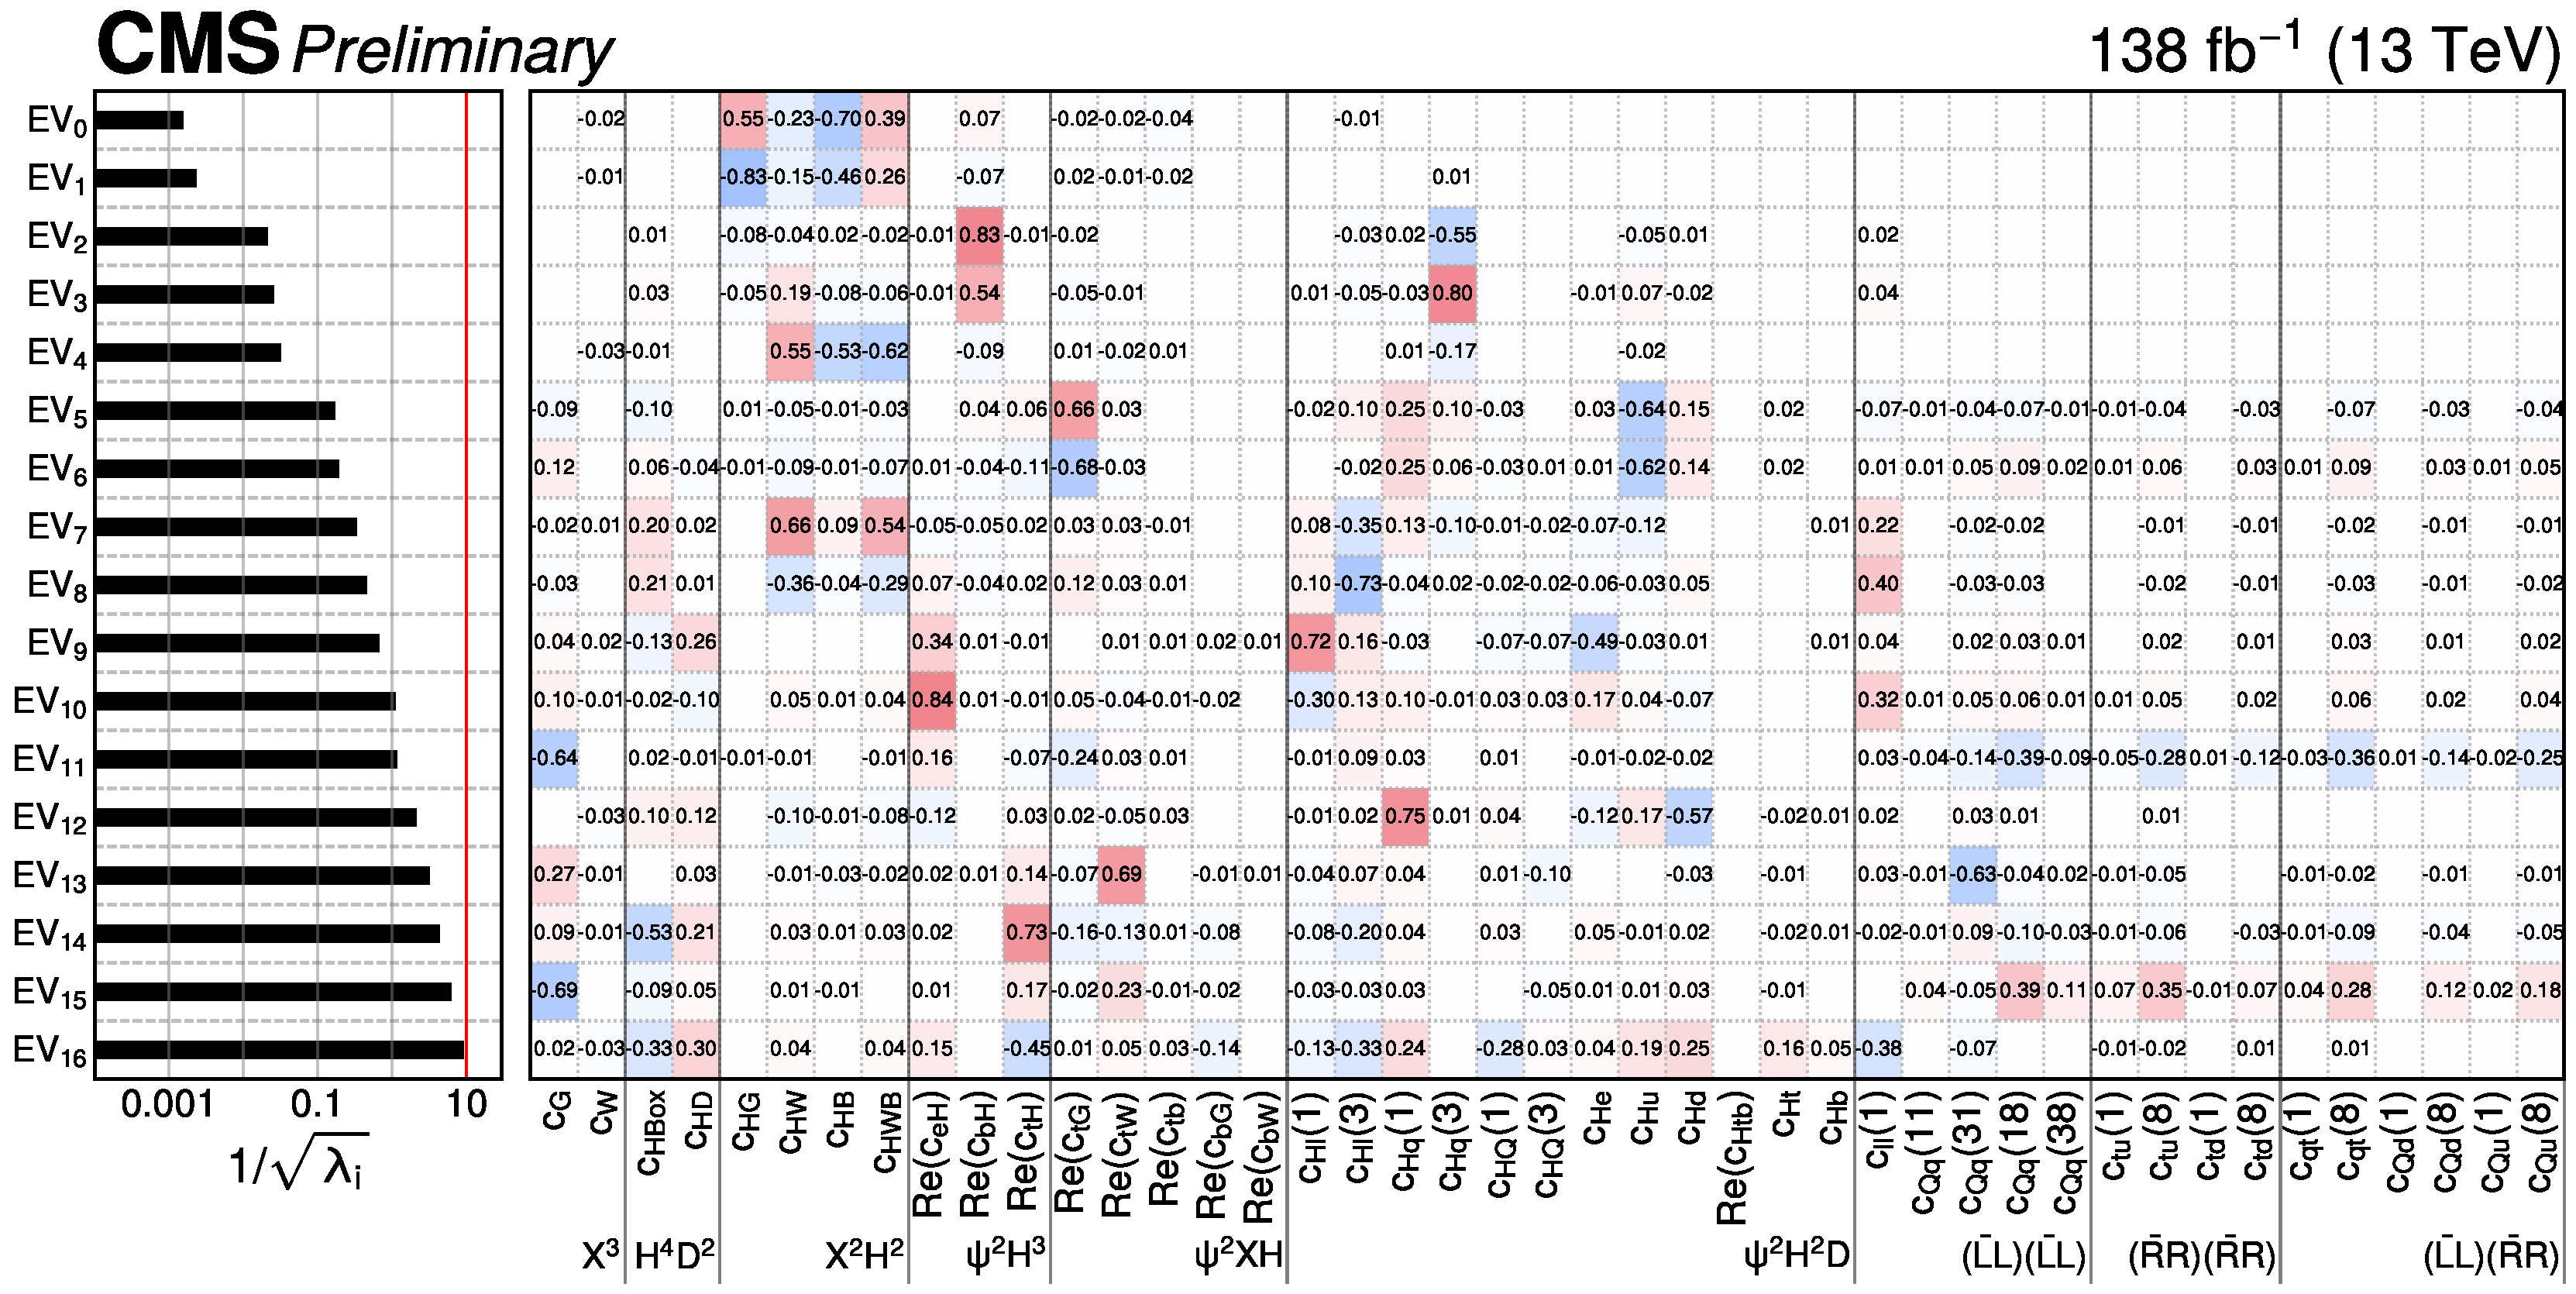
\includegraphics[width=1.1\pagewidth]{Figures/EFT/HIG-21-018-Figure_018.pdf}
    \caption[Truncated PCA Rotation Matrix]{The rotation matrix, $\mathcal{R}$, derived using the PCA procedure, truncated according to the 17 eigenvectors included in the fit to data. The values in the matrix are shown by text and a colour scale that goes from blue (negative values) to red (positive values). The left panel shows the expected 68\% CL interval given by $1/\sqrt{\lambda_i}$, where $\lambda_i$ is the eigenvalue for eigenvector $i$.}\label{fig:pca_rotation_matrix}
  \end{figure}
\end{landscape}

\begin{landscape}
  \begin{figure}
      \centering
      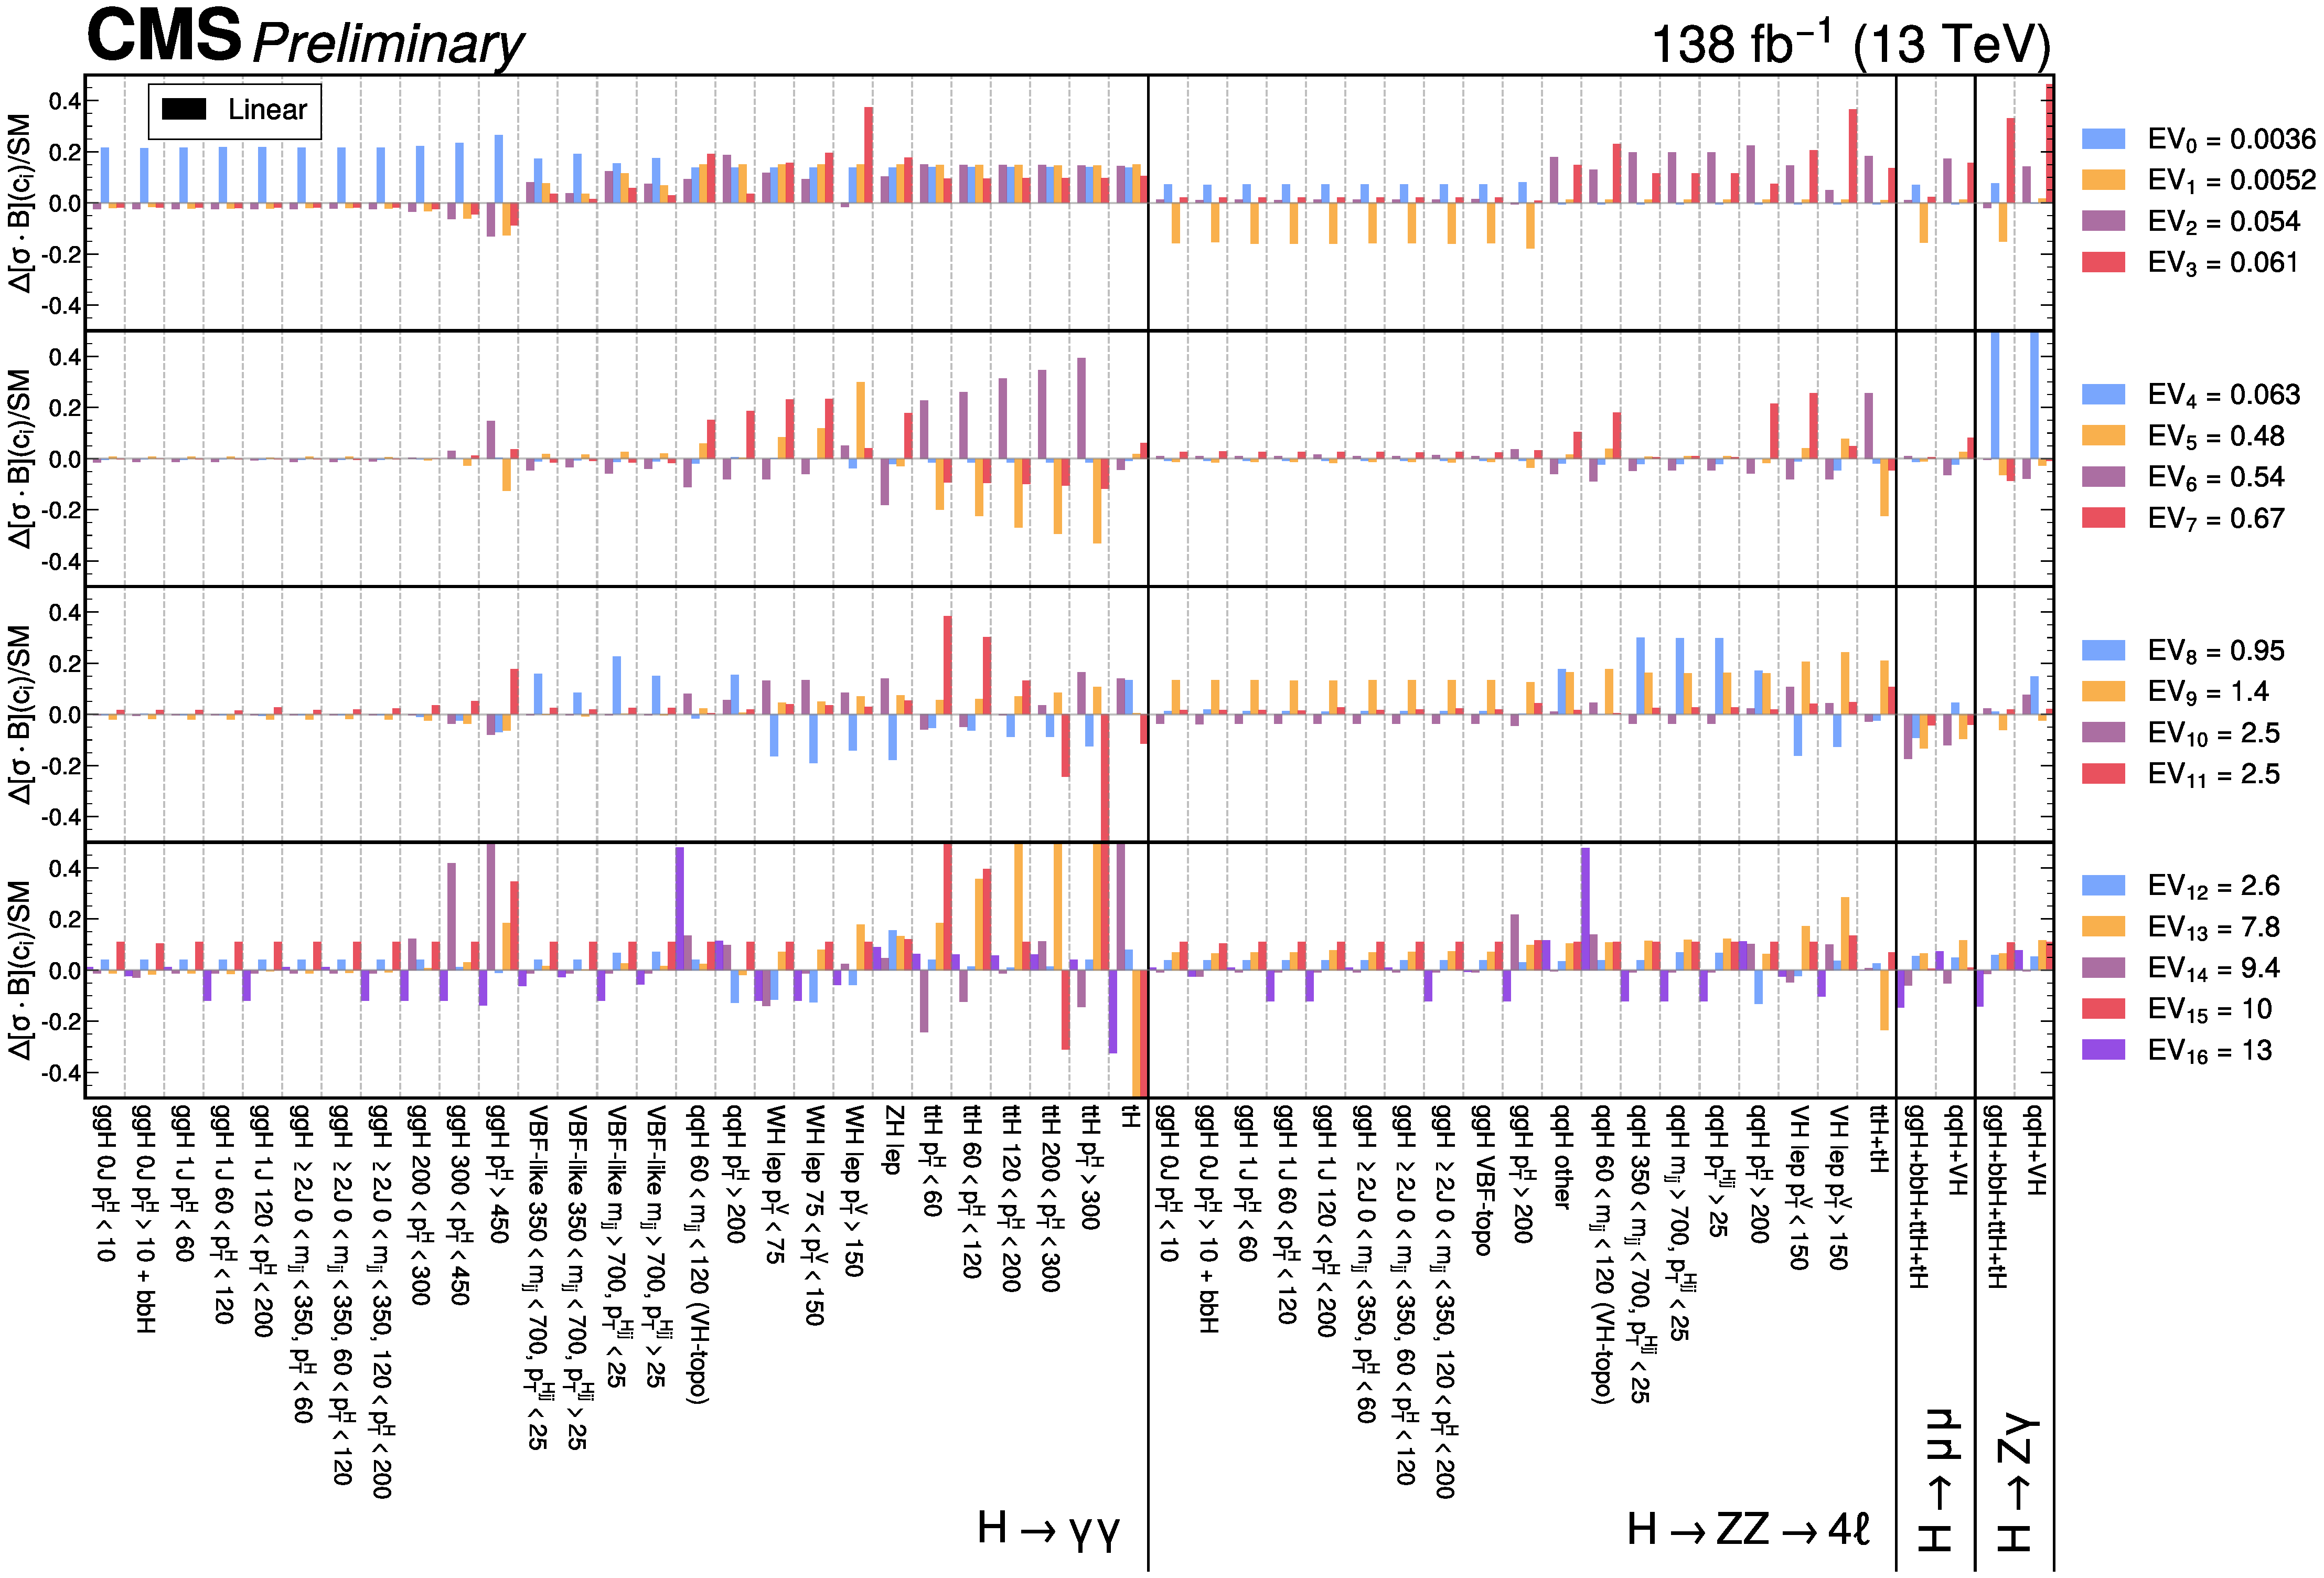
\includegraphics[width=.9\linewidth]{Figures/EFT/HIG-21-018-Figure_019.pdf}
      \caption[Impact of SMEFT Operators in the Rotated Basis (1)]{Impact of the eigenvectors on the STXS cross sections times branching fractions for the \Hgg, \Hfl, \Hmumu and \HZg decay channels. The eigenvectors are set to the expected symmetrized 95\% CL interval value in the profiled fit (when other eigenvectors are freely floating). The impacts are presented relative to the SM prediction and shown by filled bars for the linear parameterization only.}\label{fig:smeft_parametrisation_rotated_linear_part1}
  \end{figure}
\end{landscape}

\begin{landscape}
  \begin{figure}
      \centering
      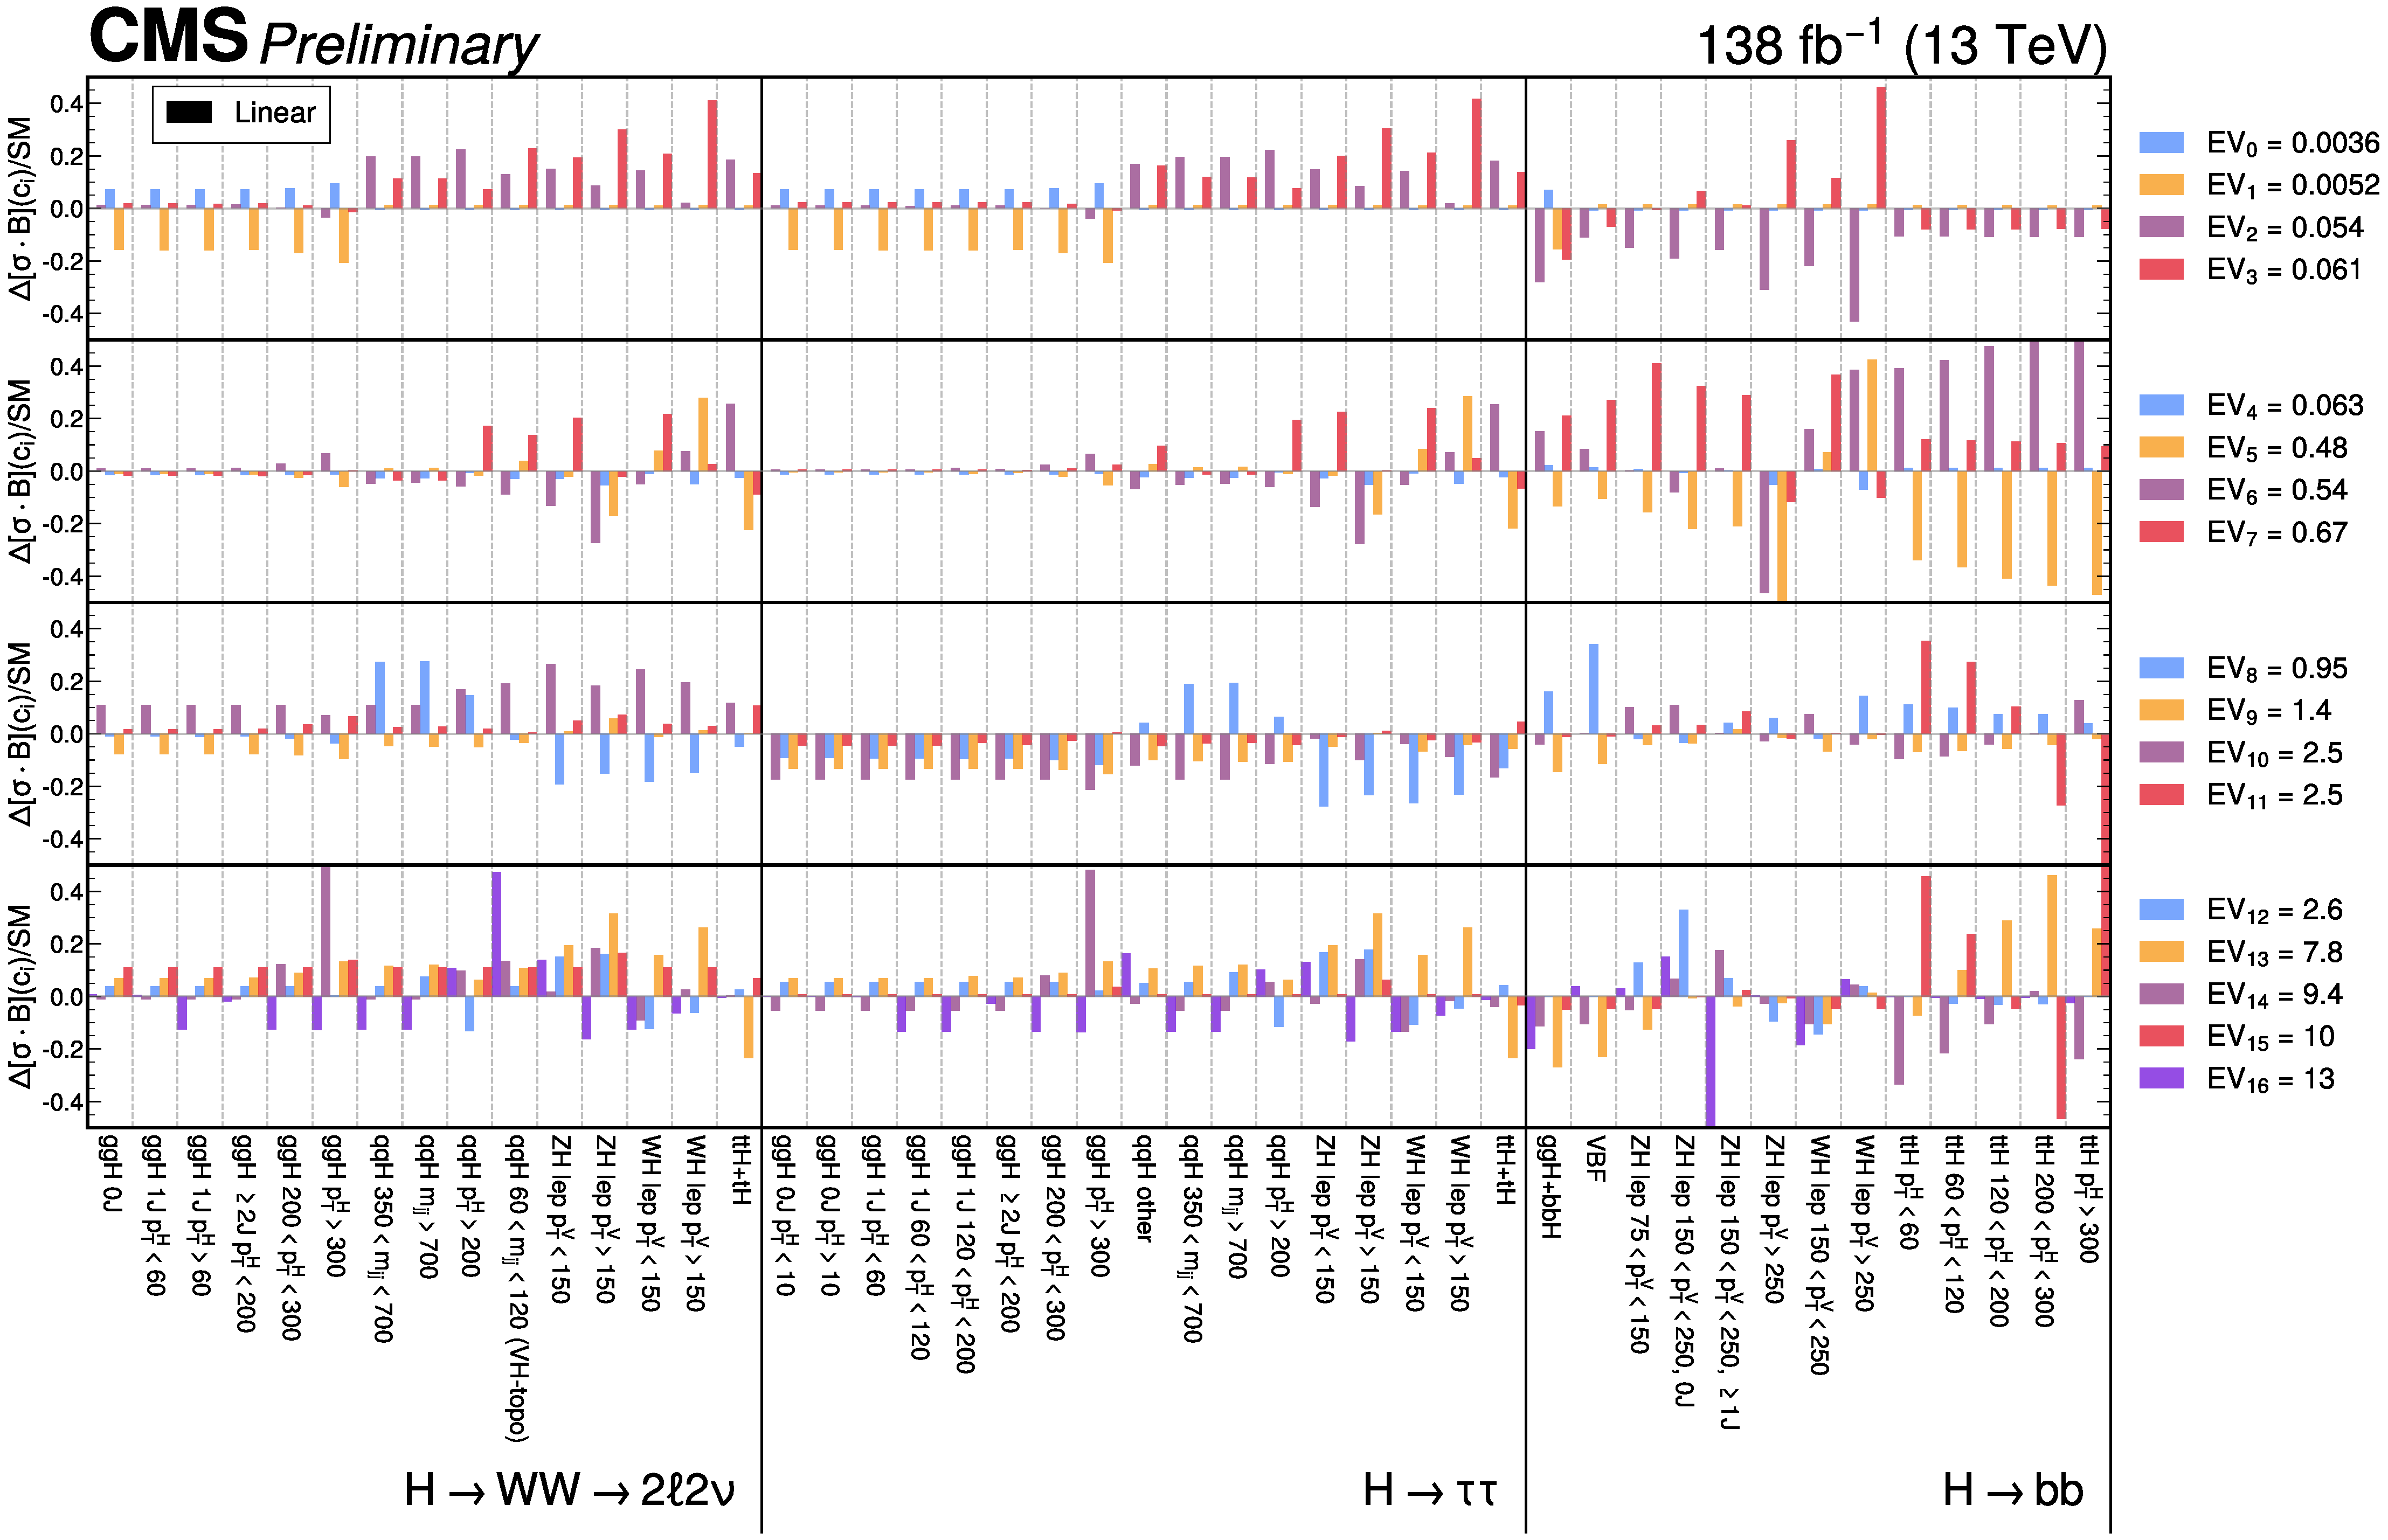
\includegraphics[width=.9\linewidth]{Figures/EFT/HIG-21-018-Figure_020.pdf}
      \caption[Impact of SMEFT Operators in the Rotated Basis (2)]{Impact of the eigenvectors on the STXS cross sections times branching fractions for the \Hlnulnu, \Htautau, and \Hbb decay channels. The eigenvectors are set to the expected symmetrized 95\% CL interval value in the profiled fit (when other eigenvectors are freely floating). The impacts are presented relative to the SM prediction and shown by filled bars for the linear parameterization only.}\label{fig:smeft_parametrisation_rotated_linear_part2}
  \end{figure}
\end{landscape}

Using these figures and the impacts in the nominal basis (\cref{fig:smeft_parametrisation_part1,fig:smeft_parametrisation_part1,fig:smeft_parametrisation_part1}), one can understand the construction of the eigenvectors and assign meaning to them. For example, the most sensitive eigenvector, $\mathrm{EV}_0$, is a combination of $C_{HG}$, which primarily affects \ggH production, and $C_{HB}$, $C_{HW}$ and $C_{HWB}$, which have the largest impact on the \Hgg branching fraction. Therefore, this eigenvector primarily affects \ggH production, specifically in the \Hgg decay channel (see \cref{fig:smeft_parametrisation_rotated_linear_part1}). It is unsurprising that this particular combination has the best expected sensitivity since inclusive measurements of \ggH and \Hgg in this combination have the smallest uncertainties when compared to other production and decay modes~\cite{CMS-PAS-HIG-21-018}. Similarly, it follows that the next eigenvector, $\mathrm{EV}_1$, primarily affects \ggH production in the other channels, and has a similar sensitivity to $\mathrm{EV}_0$.

\begin{figure}
  \centering
  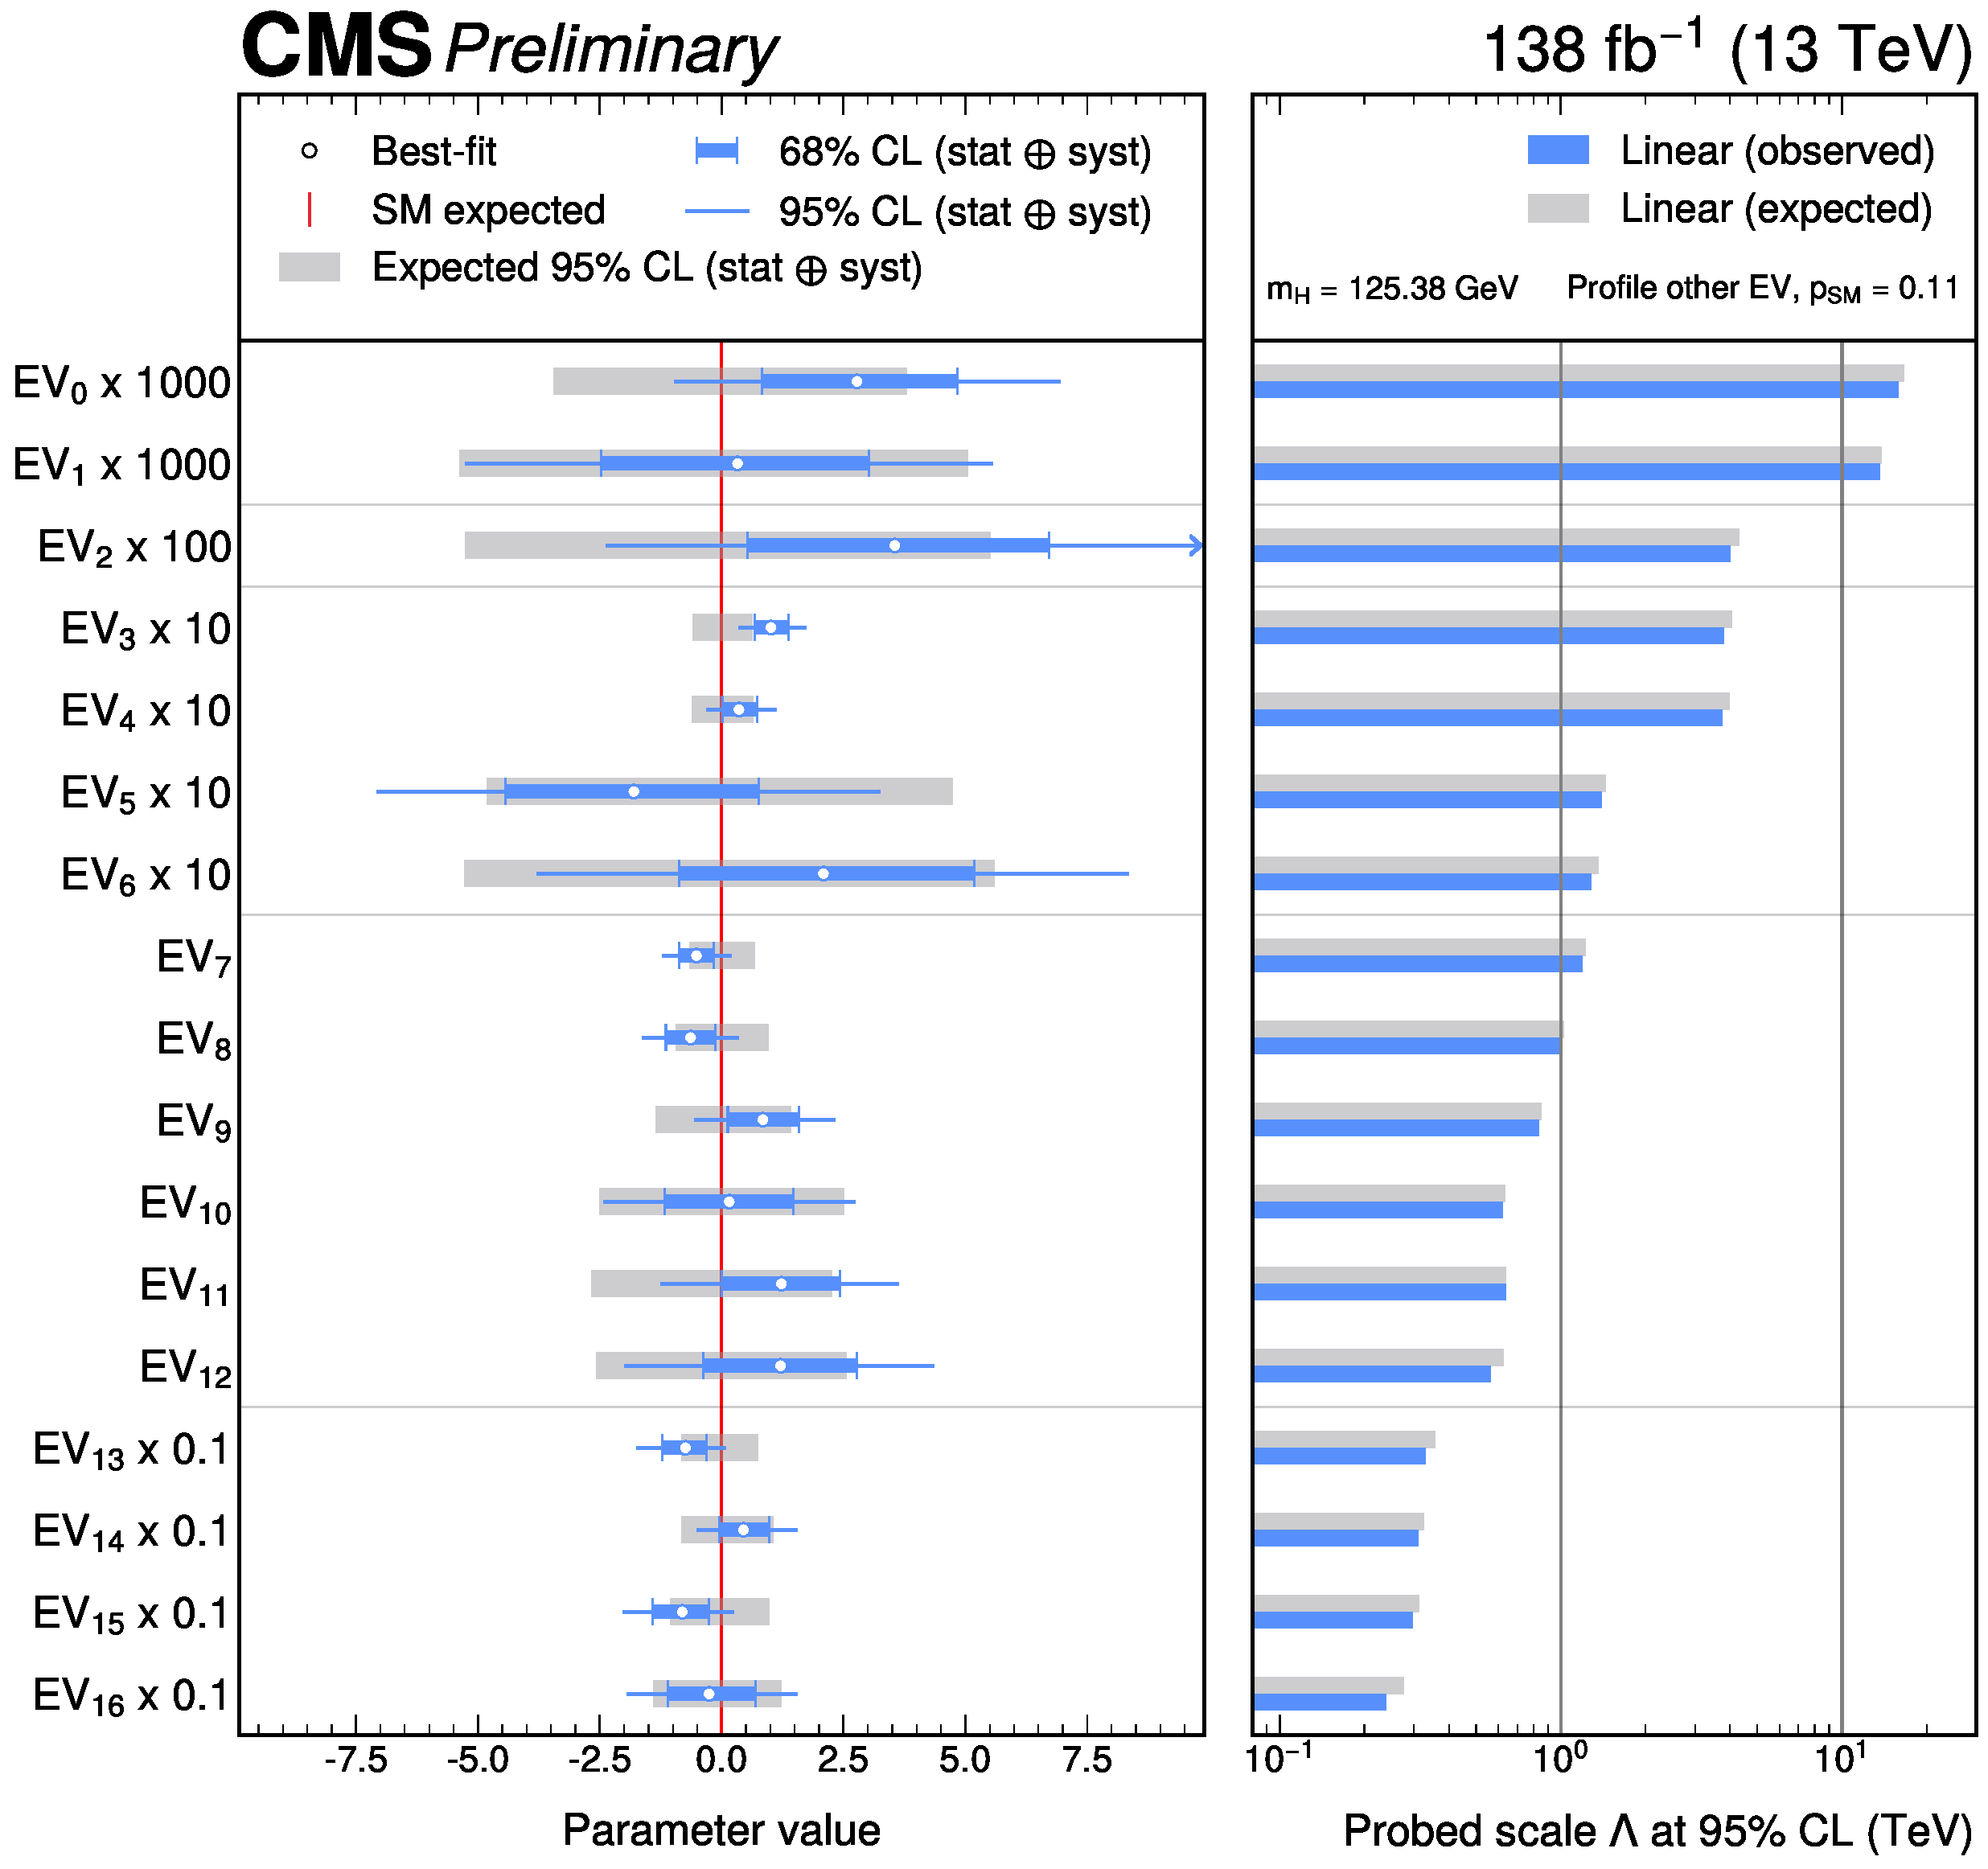
\includegraphics[width=1\textwidth]{Figures/EFT/HIG-21-018-Figure_021.pdf}
  \caption[Simultaneous Constraints on the SMEFT Eigenvectors]{Observed and expected constraints on the eigenvectors from a profiled fit where the other eigenvectors are left freely floating. The left panel shows the best-fit values, the SM expectation ($C=0$), and the 68\% and 95\% CL intervals. Only the results for the linear parameterization are shown. When a confidence interval extends beyond the range of the plot, it is indicated by an arrow. The right panel shows the 95\% CL lower limits on the probed energy scale, $\Lambda$, when assuming $c_i=1$.}\label{fig:summary_SMEFT_linearOnly}
\end{figure}

Maximum likelihood fits are used to extract 1D constraints on each of the 17 eigenvectors when allowing the other 16 eigenvectors to float freely. In these fits, only the linear parameterization is used, and this is done for several reasons. Firstly, the rotated basis is defined for the linear parameterization only and by introducing the quadratic terms, the basis is made no longer orthogonal. Secondly, the quadratic terms lead to more local minima in the NLL, causing the minimizer to struggle to find the true minimum, which in turn can lead to less reliable confidence intervals. 

Finally, including the quadratic terms corresponds to an inconsistent SMEFT expansion in powers of $1/\Lambda^2$ because the quadratic terms enter at $1/\Lambda^4$, which is the same order that dimension-8 contributions would begin to enter. This is an issue because the inclusion of quadratic terms may lead to tighter constraints, which may not hold if the dimension-8 contributions were included. Therefore, it is preferred to use the linear parameterization only, which is more conservative and may provide a more realistic indication of the sensitivity.

The expected and observed best-fit values, 68\% and 95\% CL intervals, and corresponding lower limits on the probed energies scales for the eigenvectors are shown in \cref{fig:summary_SMEFT_linearOnly}. The 95\% CL intervals range from $\pm 0.005$ to $\pm 20$ around the best-fit value depending on the eigenvector, and lower limits on the probed energy scales are up to 11\TeV and as low as 0.2\TeV.

Overall, fair agreement is found with the SM, with a p-value of 0.11. The most discrepant eigenvector is $\mathrm{EV}_3$, which is primarily a combination of $Re(C_{bH})$ and $C_{Hq}^{(3)}$. This follows from the discrepancy in $C_{Hq}^{(3)}$ seen in the nominal basis results which is explained by disagreements with the SM in measurements of the high \ptV \WH and \ZH leptonic bins. \Cref{fig:smeft_parametrisation_rotated_linear_part1,fig:smeft_parametrisation_rotated_linear_part2} show that this eigenvector has its largest impact in these particular bins as well. 